\chapter{Definici\'on del Problema}

\section{Definición}

Las proteínas desempeñan un papel fundamental para la vida y son las biomoléculas más versátiles y diversas, las cuales realizan una enorme cantidad de funciones diferentes, tales como enzimáticas, estructurales, inmunológicas, entre otras. Para muchos biólogos y científicos especializados en este tipo de biomolécula resulta crucial investigar sobre tales propiedades anteriormente mencionadas, por lo tanto para ellos es necesario saber o conocer la composición básica de cada una de las proteínas en base a su elemento básico, conocido como el aminoácido (existen 20 diferentes en total). Todas las proteínas se componen de aminoácidos, entregando así una cantidad inmensa de polipéptidos que existen y que van apareciendo gracias al trabajo de investigaciones y proyectos que hacen los encargados de este asunto.

Estas proteínas aparecen registradas en base de datos (como UniProt, Genbank o EROP-Moscow) con su secuencia, su nombre taxonómico y un código en clave también conocido como ID, las cuales están disponibles en archivos con formato \textbf{.fasta} (que pueden abrise usando un editor de texto básico) de la siguiente forma:

\begin{figure}[ht]
    \centering
    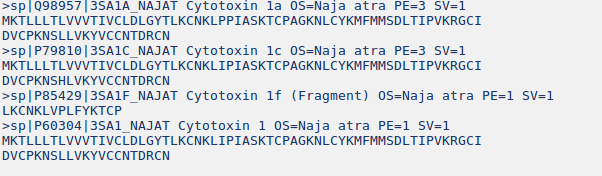
\includegraphics[width=0.8\textwidth]{./images/secuencias.png}
    \caption{Secuencias de varias proteínas en formato \textbf{.fasta}}
    \label{fig:image4}
\end{figure}

Una de las principales tareas en la investigación de proteínas consiste es buscar secuencias de aminoácidos (residuos de aminoácidos o \textit{aminoacid residues (AAR)} en inglés) en el conjunto universo de las polipéptidos para poder localizar cuáles son los residuos de ciertos tamaños que más aparecen en las bases de datos. El problema principal radica en buscar cuántas veces aparece cierto residuo de una base de datos que posean tamaños bastante considerables (por ejemplo, buscar una determinada subsecuencia de 2 aminoácidos en una base de datos de 500 GB o superior) sin saber si este residuo está presente o no en aquella base de datos, esto podría provocar gastos innecesarios de tiempo a la hora de realizar este tipo de búsqueda, por consiguiente se desea ocupar el menor tiempo posible para realizar esta tarea.

\section{Objetivos}

Lo que se pretende realizar para esta memoria consiste en obtener de un conjunto predeterminado de proteínas lo siguiente:

\begin{enumerate}

\item el número máximo de fragmentos de péptidos (AAR) que existen asociado a un valor $k$ determinado, donde $k$ se ubicará en el intervalo entre 1 hasta 50.
\item En base a lo anterior, obtener y determinar para cada $k$ cuáles son los fragmentos de aminóácidos que más se repiten.

\end{enumerate}

Una vez obtenidos estos datos se realizará un análisis algoritmico y biológico (de manera muy superficial) de los resultados logrados. Para realizar esta tarea se usarán 4 \textit{datasets}:
 
\begin{enumerate}

\item La base de datos de proteínas UniProt-SwissProt (555426 proteínas)
\item La base de datos de proteínas UniProt-TrEMBL (88032926 proteínas).
\item La base de datos de péptidos EROP-Moscow (14875 oligopéptidos).
\item Las proteínas humanas ingresadas manualmente a la base de datos UniProt (datos extraídos de UniProt-SwissProt, 86298 proteínas). Para este caso solo se considerará $k=1$.

\end{enumerate}

A partir de esto las implementaciones de código para trabajar estos archivos serán realizados en los lenguajes de programación {\textbf{C++}} y {\textbf{Python}} para ciertos gráficos y estadísticas de resultados, con diferentes finalidades que serán explicadas a medida que se avance en el documento.